\documentclass[12pt]{article}
\usepackage{graphicx}
%\documentclass[journal,12pt,twocolumn]{IEEEtran}
\usepackage[none]{hyphenat}
\usepackage{graphicx}
\usepackage{blindtext}
\usepackage{multicol}
\usepackage{listings}
\usepackage[english]{babel}
\usepackage{graphicx}
\usepackage{caption}
\usepackage[parfill]{parskip}
\usepackage{hyperref}
\usepackage{gensymb}
\usepackage{commath}
\usepackage{amssymb}
\usepackage{amsthm}
\usepackage{tikz}
\usepackage{booktabs}
\usepackage{tabularx}
\usepackage{multirow}
%\usepackage{setspace}\doublespacing\pagestyle{plain}
\def\inputGnumericTable{}
\usepackage{color}                                            %%
    \usepackage{array}                                            %%
    \usepackage{longtable}                                        %%
    \usepackage{calc}                                             %%
    \usepackage{multirow}                                         %%
    \usepackage{hhline}                                           %%
    \usepackage{ifthen}
\usepackage{array}
\usepackage{amsmath}   % for having text in math mode
\usepackage{parallel,enumitem}
\usepackage{listings}
\lstset{
language=tex,
frame=single,
breaklines=true
}
 
%Following 2 lines were added to remove the blank page at the beginning
\usepackage{atbegshi}% http://ctan.org/pkg/atbegshi
\AtBeginDocument{\AtBeginShipoutNext{\AtBeginShipoutDiscard}}
%
%New macro definitions
\newcounter{matchleft}\newcounter{matchright}

\newenvironment{matchtabular}{%
  \setcounter{matchleft}{0}%
  \setcounter{matchright}{0}%
  \tabularx{\textwidth}{%
    >{\leavevmode\hbox to 1.5em{\stepcounter{matchleft}\arabic{matchleft}.}}X%
    >{\leavevmode\hbox to 1.5em{\stepcounter{matchright}\alph{matchright}.}}X%
    }%
}{\endtabularx}
\newcommand{\mydet}[1]{\ensuremath{\begin{vmatrix}#1\end{vmatrix}}}
\providecommand{\brak}[1]{\ensuremath{\left(#1\right)}}
\providecommand{\norm}[1]{\left\lVert#1\right\rVert}
\newcommand{\solution}{\noindent \textbf{Solution: }}
\newcommand{\myvec}[1]{\ensuremath{\begin{pmatrix}#1\end{pmatrix}}}
\providecommand{\abs}[1]{\left\vert#1\right\vert}
\providecommand{\pr}[1]{\ensuremath{\Pr\left(#1\right)}}
\let\vec\mathbf
\begin{document}
\begin{center}
\enlargethispage{-4cm}
\title{\textbf{Conic Sections}}
\date{\vspace{-5ex}} %Not to print date automatically
\maketitle
\end{center}
\setcounter{page}{1}
\section*{11$^{th}$ Maths - Chapter 11}
\textbf{Short Answer Type Questions}
\begin{enumerate}
\item If the letters of the word ALGORITHM are arranged at random in a row what is the probability the letters GOR must remain together as a unit?
\item Six new employees, two of whom are married to be assigned six desks that are lined up in a row. lf the assignment of employees to desks is made randomly, what is the probability that the married couple will have nonadjacent desks:
[Hint: First find the probability that the couple has adjacent desks, and then subtract it from 1.]
\item Suppose an integer from 1 through 1000 is chosen at random, find the probability that the integer is a multiple of 2 or a multiple of a
\item An experiment consists of rolling a die until a 2 appears.
\item How many elements of the sample space correspond to the event that the 2 appears on the $k^{th}$ roll of the die?
	[Hint:(a) First (k-1) rolls have 5 outcomes each and $k^{th}$ rolls should result in 1 outcomes. (b) 1+5+$5^2$+....+$5^{k-1}$].
\item A die is loaded in such a way that each odd number is twice as likely to occer as each even number. Find $\pr{G}$, where $G$ is the event that a number greater than 3 occurs on a  single rall of the die
\item In a large metropolitan area, the probabilities are .87, .36, .30 that a family (randomly chosen for a sample survey) owns a colour television set, a block and white television set, or both kinds of sets what is the probability that a family owns either any one or both kinds of sets
\item  If $A$ and $B$ are mutually exclusive events. $\pr{A}=0.35$ and $\pr{B}=0.45$ find
\begin{enumerate}
\item $\pr{A}$
\item $\pr{B}$
\item $\pr{A\cup B}$
\item $\pr{A\cap B}$
\item $\pr{A\cap B}$
\item ${A\prime\cap B\prime}$
\end{enumerate}
\item A team of medical students doing their internship have to assit during sur geries at a city hospital. The probabilities of surgeries rated as very complex. Complex, routine, simple or very simple are respectively, 0.15,0.20,0.31,0.26,.08. Find the probabilities that a pariticular surgery will be rated
\begin{enumerate}
\item complex or very complex.
\item neither very complex nor very simple.
\item routine or complex. 
\item routine or simple.
\end{enumerate}
\item Four candidates $A,B,C,D$ have applied for the assignment to coach a school cricket team .If $A$ is twice as likely to be selected as $B$, and $B$, and $B$ and $C$ are given about the same chance of being selected. while $C$ is twice as likely to be selected as $D$, what are the probabilities that
\begin{enumerate}
\item $C$ will be selected ?
\item $A$ will not be selected ?
\end{enumerate}
\item One of the four persons John, Rita, Aslam or Gurpreet will be promoted next month. Consequently the sample space consists of four elementary outcomess=[John promoted, Rita promoted, Aslam promoted, Gurpreet promoted] you are told that the chances of John's promotion is same as that of Gurpreet, Rita's chances of promotion are twice as likely as Johns. Aslam's chances are four times that of John.
\begin{enumerate}
\item Determine $\pr{John promoteg}$
$\pr{Rita promoted}$
$\pr{Aslam promoted}$
$\pr{Gurpreet promoted}$
\item If $A$ ={John promoted or Gurpreet promoted} find $\pr{A}$.
\end{enumerate}
\item The accompanying venn diagram shows three events $A,B$ and $C$, and also the probabilities of the various intersections (for instance. $\pr {A\cap B} =0.7$). Determine
\begin{figure}[h!]                                   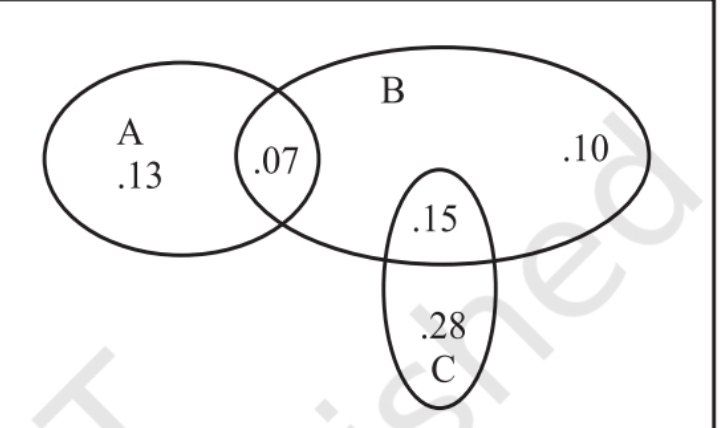
\includegraphics[width=\columnwidth]{figs/pic.jpg}                           \caption{}                                       \label{fig:1}                    \end{figure}
	\begin{enumerate}
	\item $\pr {A}$
	\item $\pr {B \cap C}$
	\item $\pr {A\cap B}$
	\item $\pr {A\cap B}$
	\item $\pr {A\cap B}$
	\item $\pr {B\cap C}$
\end{enumerate}
\item Probability of exactly one of the three occurs.
\item One urn contains two black balls (labelled $B1$ and $B2$) and one white ball and two white balls (labelled $W1$ and $W2$). Suppose the  following experiment is performed one of the two urns is chosen at random. newt a ball is randomly chosen from the urn. Then a second ball is chosen at random from the some urn without replacing the first ball.
	\begin{enumerate}
		\item Write the sample space showing all possible outcomes.
\item What is the probability that two black balls are chosen?
\item What is the probability that two balls of opposite colour are chosen
	\end{enumerate}
\item A bag cantains 8 red and 5 white balls Three balls are drawn at random Find the probability that 
\begin{enumerate}
\item All the three balls are white
\item All the three balls are red
\item one ball is red and two balls are white
	\end{enumerate}
\item If the letters of the word ASSASSINATION are arranged at  random. Find the probabiliy that
\begin{enumerate}
\item Four 5's come consecutively in the word
\item Two 1'$s$ and two $N' S$  come together
\item All A'S are not coming together
\item No two A's are coming together
	\end{enumerate}
\item A card is drawn from a deck of 52 cards Find the probability of getting aking or a heart or a red card.
\item A sample space consists of a elementary outcomes $e_1,e_2,....,e_9$ whose probabilities are
 $\pr{e_1}=\pr{e_2}=0.8,\pr{e_4}=\pr{e_4}=\pr{e_5}=.1$

$\pr{e_6}=\pr{e_7}=.2,\pr{e_9}=0.7$

Suppose $A={e_1,e_5,e_8},B={e_2,e_5,e_8,e_9}$
\begin{enumerate}
\item calculate $\pr {A},\pr{B}$,and $\pr {A\cap B}$
\item Using the addition law of probability. Calcuate $\pr {A\cap B}$
\item List the composition of the event $A\cap B$, and calcutate $\pr {A\cap B}$ by adding the probabilities of the elementary outcomes
\item calcuate $\pr {\overline{B}}$ from $\pr {B}$, also calculate $\pr {\overline{B}}$ directly from the elementary outcomes of $\overline{B}$
\end{enumerate}
\item Determine the probability, for each of the following events 
	\begin{enumerate}
\item An odd number appears in a single toss of a fair die
\item At least one head appears in two tosses of a fair coin 
\item A king, 9 of hearts, or 3 of spades appears in drawing a single card froma well shuffled ordinary deck of 52 cards
\item The sum of 6 appears in a single toss of a pair of fair dice
	\end{enumerate}
	\end{enumerate}
\textbf{Objective Type Questions}

Choose the corrent answer out of four given options in each of the exercises 18 to 29(M.C.Q)
\begin{enumerate}[resume]
\item In a non-leap year. The probability of having 53 tuesdays or 53 wednesdays is
\begin{enumerate}
\item $\frac{1}{7}$
\item $\frac{2}{7}$
\item $\frac{3}{7}$
\item none of these
\end{enumerate}
\item Three numbers are chosen from 1 to 20- Find the probability that they are not consecutive
\begin{enumerate}
\item $\frac{186}{190}$
\item $\frac{187}{190}$
\item $\frac{188}{190}$
\item $\frac{18}{20\cap3}$
\end{enumerate}
\item While shuffing a pack of 52 playing cards, 2 are accidentally dropped. Find the probability that the missing cords to be of different colours.
\begin{enumerate}
\item $\frac{29}{52}$
\item $\frac{1}{2}$
\item $\frac{26}{51}$
\item $\frac{27}{51}$
\end{enumerate}
\item seven persons are to be seated in a row The probability that two particular persons sit next to each other is
\begin{enumerate}
\item $\frac{1}{3}$
\item $\frac{1}{6}$
\item $\frac{2}{7}$
\item $\frac{1}{2}$
\end{enumerate}
\item Without repetitin of the numbers four digit numbers are  formed with the numbers 0,2,3,5. The probability of such a numbers divisible by 5 is
\begin{enumerate}
\item $\frac{1}{5}$
\item $\frac{4}{5}$
\item $\frac{1}{30}$
\item $\frac{5}{9}$
\end{enumerate}
\item If $A$ and $B$ are mutually exclusive events, then
\begin{enumerate}
	\item $\pr{A}<\pr{B}$
	\item $\pr{A}>\pr{B}$
	\item $\pr{A}<\pr{B}$
\item none of these
\end{enumerate}
\item If $\pr {A\cap B}=\pr{A\cap B}$ for any two events $A$ and $B$, then 
\begin{enumerate}
	\item $\pr{A}=\pr{B}$
	\item $\pr{A}>\pr{B}$
	\item $\pr{A}<\pr{B}$
\item none of these
\end{enumerate}
\item 6 boys and 6 girls sit in a row at random. The probability that all the girls sit together is
\begin{enumerate}
\item $\frac{1}{432}$
\item $\frac{12}{431}$
\item $\frac{1}{132}$
\item none of these
\end{enumerate}
\item A single letter is selected at random from the word, PROBABILITY', The probability that it is a vowel is
\begin{enumerate}
\item $\frac{1}{3}$
\item $\frac{4}{11}$
\item $\frac{2}{11}$
\item $\frac{3}{11}$
\end{enumerate}
\item If the probabilities for $A$ to fail in an examination is 0.2 and that for $B$ is 0., then the probability that either $A$ or $B$ fails is
\begin{enumerate}
\item $>$ 5 
\item .5
\item $<$.5
\item 0
\end{enumerate}
\item The probability that at least one of the events $A$ and $B$ occurs is 0.6. If $A$ and $B$ occur simultaneously with probability 0.2, then $\pr{A}+\pr{B}$ is 
\begin{enumerate}
\item 0.4
\item 0.8
\item 1.2
\item 1.6
\end{enumerate}
\item If $M$ and $N$ are any two events, the probability that at least one of them occurs is
\begin{enumerate}
	\item $\pr{M}+\pr{N}-2 \pr {M\cap N}$
	\item $\pr{M}+\pr{N}-\pr{M\cap N}$
	\item $\pr{M}+\pr{N}\pr{M\cap N}$
	\item $\pr{M}+\pr{N}+2\pr{M\cap N}$
\end{enumerate}
\item The probability that a person visiting a 200 will see the giraffee is 0-72. the probability that he will see the bears is 0.84 and the probability that he will see both is 0.52.
\item The probability that a student will pass his examination is 0.73, the probability of the student getting a compartment is 0,13, and the probability that the student will cither pass or get compartment is 0.96.
\item The probabilitiesthat a typist will make 0,1,2,3,4,5 or more mistakes in typing areport are, respectively, 0.12,0,25,0.36, 0.14.0.08,0.11.
\item If $A$ and $B$ are two candidates seeking admission in an engineering college. The probability that both $A$ and $B$ are selected is at most. 3 ls it possible that the probility of $B$ getting selected is0.7 ?
\item The probability of intersection of two events $A$ and $B$ is always less than or equal to those favourable to the evant $A$
\item The probability of an occurrence of event $A$ is.7 and that of the occurrence of event $B$ is 3. and the probability of occurrence of both is 4.
\item The sum of probabilities of two students getting distinction in their final examinations is 1.2. 
Fill in the blanks in the exercises 37 to 41. 
\item The probabliity that the home team will win an upcoming footboll game is 0.77, the probability that it will tie the game is 0.08, and the probability that it will lose the game is     
\item If $e_1 ,e_2, e_3, e_4$ are the four elementary out comes in a sample space and \pr (e,)=.1 '\pr ($e_3$)=.1, then the probability of e4 is
\item Let s ={1.2,3,4,5,6} and E={11,3,5}, then E
\item If $A$ and $B$ are two events associated  with a random experiment such that $\pr{A}=0.3, \pr{B}=0.2, \pr {A\cap B}=0.1$ then the value of $\pr{A\cap B}$ is
\item The probability of happening of an event $A$ is 0.5 and that of $B$ is 0.3 lf $A$ and $B$ are mutually exclusive events, then the probability of neither $A$ nor $B$ is
%\begin{enumerate}[resume]
\item Match the proposed probability under column $C_1$, with the appropriate written descripitio under column $C_2$
\begin{table}[htbp]
 \begin{center}
    \begin{tabular}{|l|c|c|c|c|c} \hline \textbf{C1(Probablilty)}
  & \textbf{C2(Written Description)}  \\ \hline
     a) 0.95 & (i) An incoorect assignment\\ 
     b) 0.02 & (ii) No chance of happening\\ 
     c) -0.3 & (iii) As much chance of happening as not.\\
     d) 0.5 & (iv) Very likely to happen\\ 
     e) 0 & (v) Very little chance of happening\\ \hline
\end{tabular}   
\end{center}
\caption{\label{table:dummytable} }
\end{table}
%\end{enumerate}
%\begin{enumerate}[resume]
\item Match the following
\begin{table}[htbp]
 \begin{center}
    \begin{tabular}{|l|c|c|c|c|c} \hline \textbf{Column C1}
  & \textbf{Column C2}  \\ \hline
     1. If E1 , and E2 are the two
mutually exclusive evets & a.  $E_1\cap E_2=E_1$\\ 
     2. If E1 , and E2 are the two
mutually exclusive events & b. $(E_1,-E_2)\cap (E_1,\cap E_2)=E_1$\\ 
     3. If E1 , and E2 have common out
comes, then & c.  $E_1,\cap E_2=\phi,E_1,\cap E_2=S$\\
     4. If E1 and E2 are two events such that E1$\subset$ E2 & d. $E_1\cap E_2=\phi$\\  \hline
\end{tabular}   
\end{center}
\caption{\label{table:dummy} }
\end{table}
%\end{enumerate}
\end{enumerate}
\end{document}
